\documentclass{beamer}
\title{Retainer topic indexing}
\author{Ilya Averyanov}
\institute{EMQX}
\date{2022}
\usetheme{emqx}
\usepackage{listings}
\usepackage{color}
\usepackage{graphicx}
\usepackage{xcolor}
\usepackage{hyperref}
\definecolor{href}{rgb}{0,0,0.9375}
\hypersetup{
    pdfborderstyle={/S/U/W 1}, % underline links instead of boxes
    colorlinks=true,
    urlcolor=href
}
\lstset{frame=tb,
  aboveskip=3mm,
  belowskip=3mm,
  showstringspaces=false,
  columns=flexible,
  basicstyle={\small\ttfamily},
  numbers=none,
  numberstyle=\tiny\color{gray},
  keywordstyle=\color{blue},
  commentstyle=\color{dkgreen},
  stringstyle=\color{mauve},
  breaklines=true,
  breakatwhitespace=false,
  tabsize=2
}


\begin{document}

\frame{\titlepage}

\begin{frame}
    \frametitle{Retaining feature}

    \begin{center}
        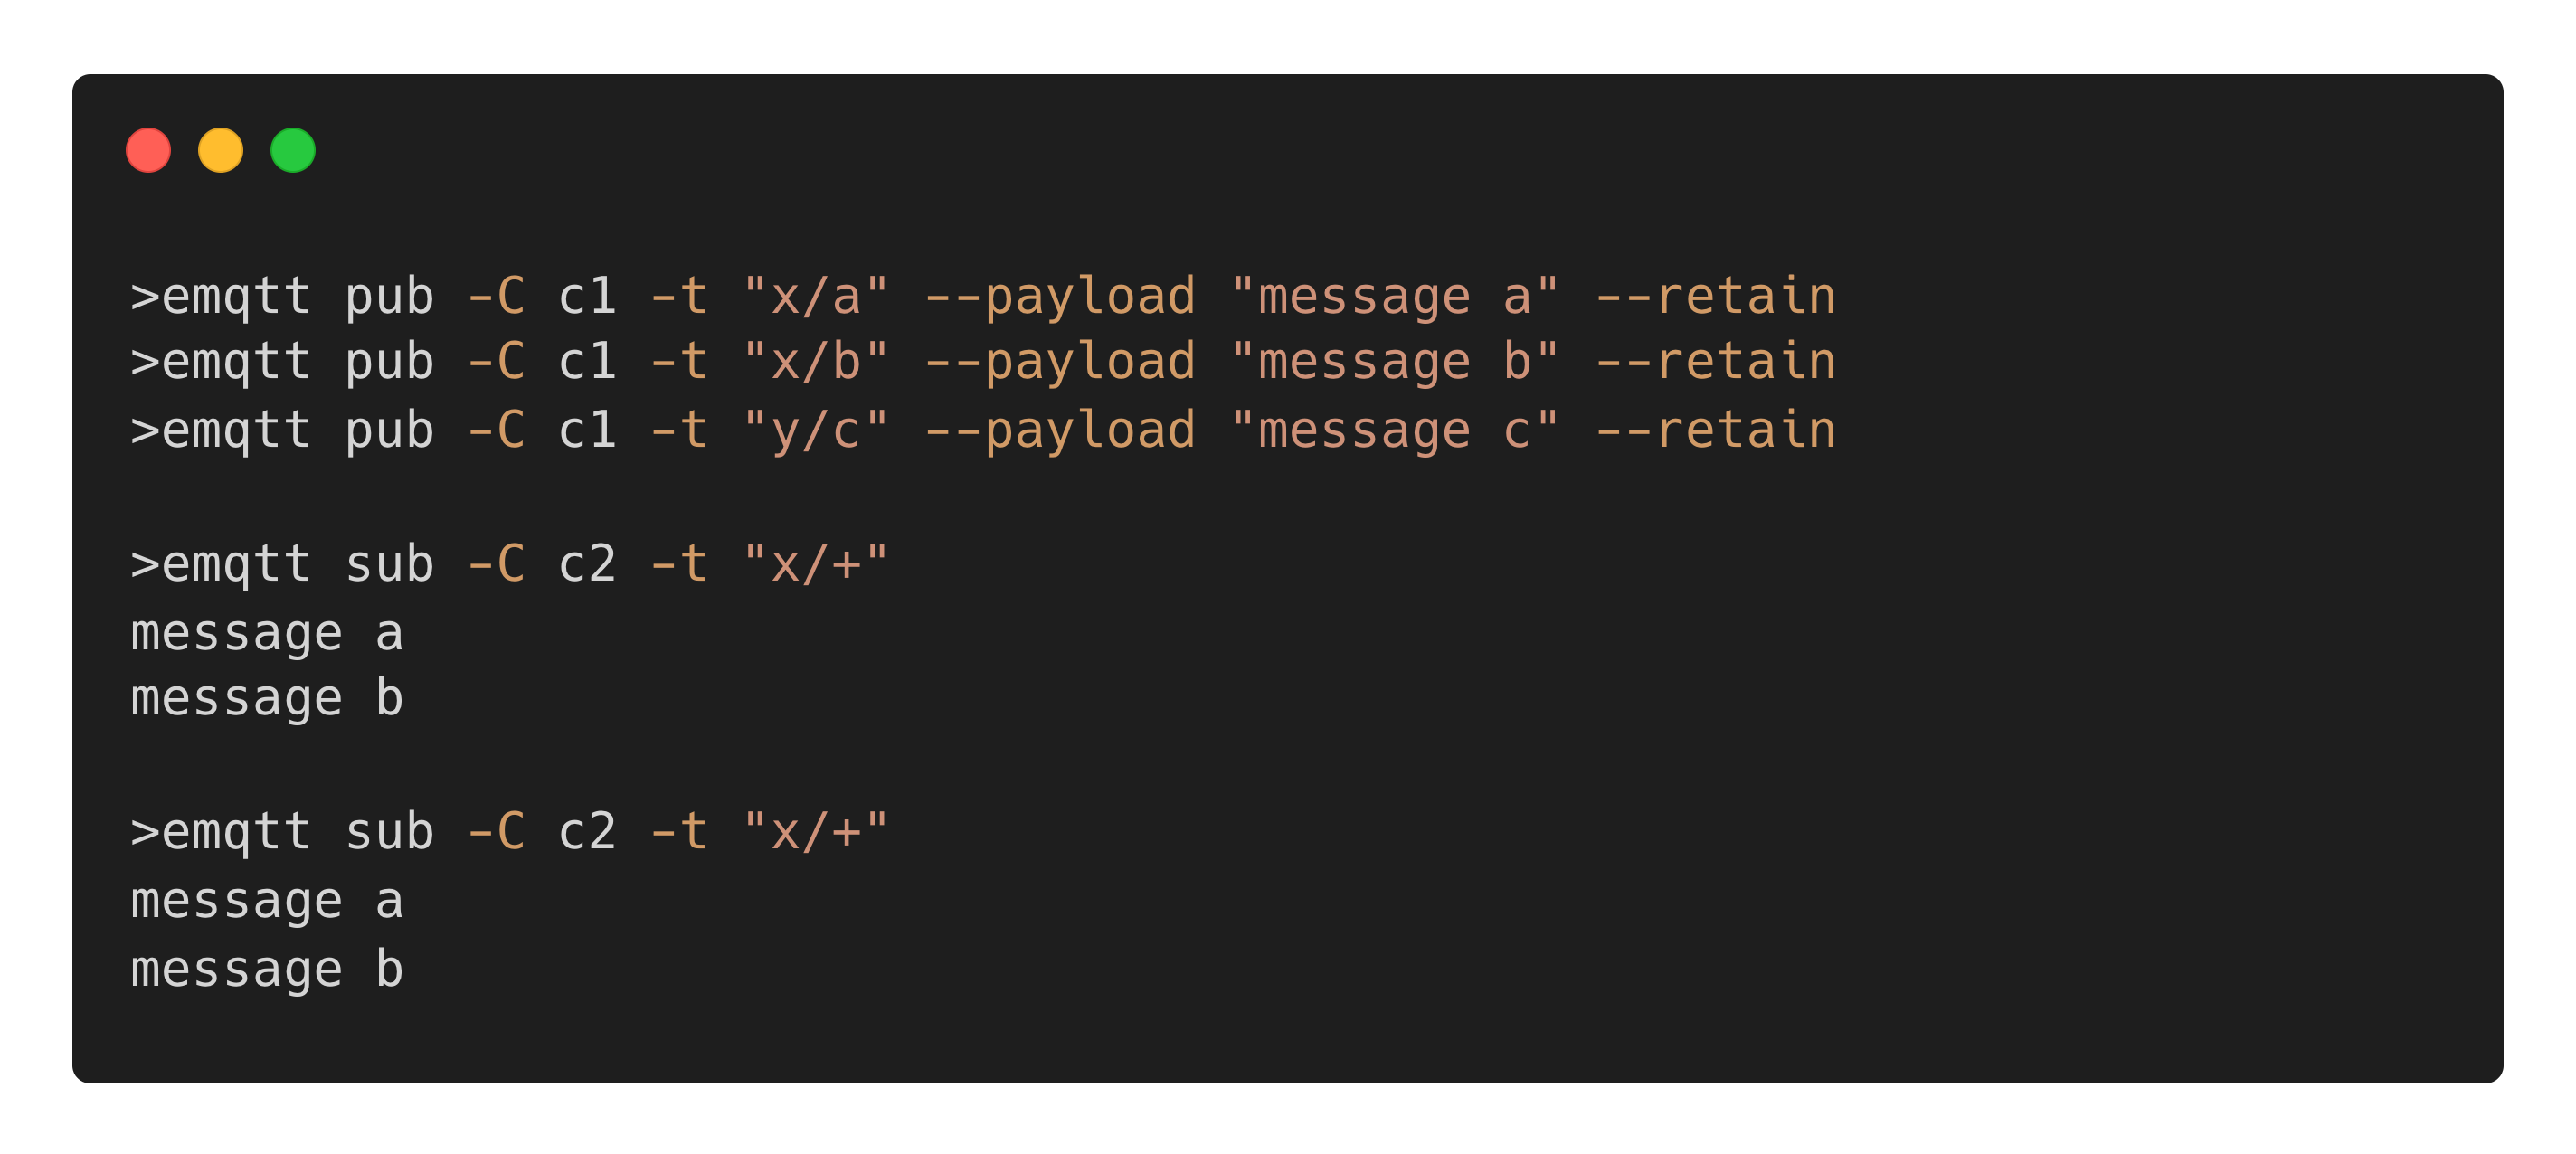
\includegraphics[width=10cm, keepaspectratio]{images/retain-demo.png}
    \end{center}
\end{frame}

\begin{frame}
    \frametitle{Retaining feature}
    \framesubtitle{Externally}

    \begin{itemize}
        \item Each topic can have a "retained" message
        \item This message is sent to each subscriber on topic subscribe
        \item A subscriber can subscribe to many topics at once using wildcards and receive many
        retained messages
    \end{itemize}
\end{frame}

\begin{frame}
    \frametitle{Retaining feature}
    \framesubtitle{Internally}

    \begin{itemize}
        \item A broker needs to keep a "database" of topics and their corresponding retained messages
        \item On topic subscribe, a broker makes a lookup of corresponding retained messages
    \end{itemize}
\end{frame}

\begin{frame}
    \frametitle{Retainer database}
    \framesubtitle{Internally}

    \begin{itemize}
        \item A subscribed topic can be "concrete", like \lstinline{a/b/c/d}.
        Then we need a simple lookup in a key-value storage to find a retained message
        \item A subscribed topic can be a wildcard topic, like \lstinline{+/b/+/d}. Then
        we first need to select relevant topics and only
        then lookup the corresponding retained messages
        \item There may be a lot of topics with retained messages so selecting relevant
        topics may be resourse consuming
        \href{https://github.com/emqx/emqx/issues/6014}{https://github.com/emqx/emqx/issues/6014}
    \end{itemize}
\end{frame}

\begin{frame}
    \frametitle{Retainer indexing}
    \framesubtitle{Solution}

    To provide effective topic search we introduce topic indexing.

    Topic indexing allows to specify topic segment positions that are supposed
    to be meaningful and not wildcard during subscriptions.

    Retained messages will be searched effectively during such subscriptions.
\end{frame}

\begin{frame}
    \frametitle{Retainer indexing}
    \framesubtitle{Example}

    Assume we have the following topic structure:

    \lstinline{<Country>/<City>/<Office>/<DeviceModel>/<Owner>}

    \vspace{1cm}

    For example:

    \lstinline{UK/London/HQ/ModelA/User4534}

\end{frame}

\begin{frame}
    \frametitle{Retainer indexing}
    \framesubtitle{Example}

    We want to subscribe to topics corresponding to some particular
    \lstinline{DeviceModel} and \lstinline{Owner}.

    \vspace{1cm}

    The wildcard will be:
    \lstinline{+/+/+/<DeviceModel>/<Owner>}
\end{frame}

\begin{frame}[fragile]
    \frametitle{Retainer indexing}
    \framesubtitle{Example}

    To optimize finding retained messages for such a subscription
    we can specify the following index:

    \vspace{1cm}
    \begin{lstlisting}

        retainer {
            backend {
                ...
                index_specs = [ [4, 5] ]
            }
        }
    \end{lstlisting}
\end{frame}

\begin{frame}[fragile]
    \frametitle{Retainer indexing}
    \framesubtitle{Notes}

    \begin{itemize}
        \item By default there are indices that help to handle wilcard subscriptions
        having any meaningful segments in the first 3 positions
        \item To enable new indices after config change one should explicitly run reindex:
        \lstinline{emqx_ctl retainer reindex start}
    \end{itemize}
\end{frame}

\begin{frame}
    \begin{center}
        Thank you!
    \end{center}
\end{frame}

\end{document}
